\documentclass[11pt]{article}

\usepackage{ucs}
\usepackage{graphicx}
\usepackage[T1]{fontenc}
\usepackage[utf8x]{inputenc} 
\usepackage[russian]{babel}
\usepackage{amssymb, amsfonts, amsmath, mathtext, cite, enumerate, float}
\usepackage{geometry}
\usepackage{fancyhdr}

\geometry{left=2cm}
\geometry{right=1.5cm}
\geometry{top=2cm}
\geometry{bottom=2cm} 

\newcommand\measurepage{\dimexpr\pagegoal-\pagetotal-\baselineskip\relax}

\newcommand\fillpage{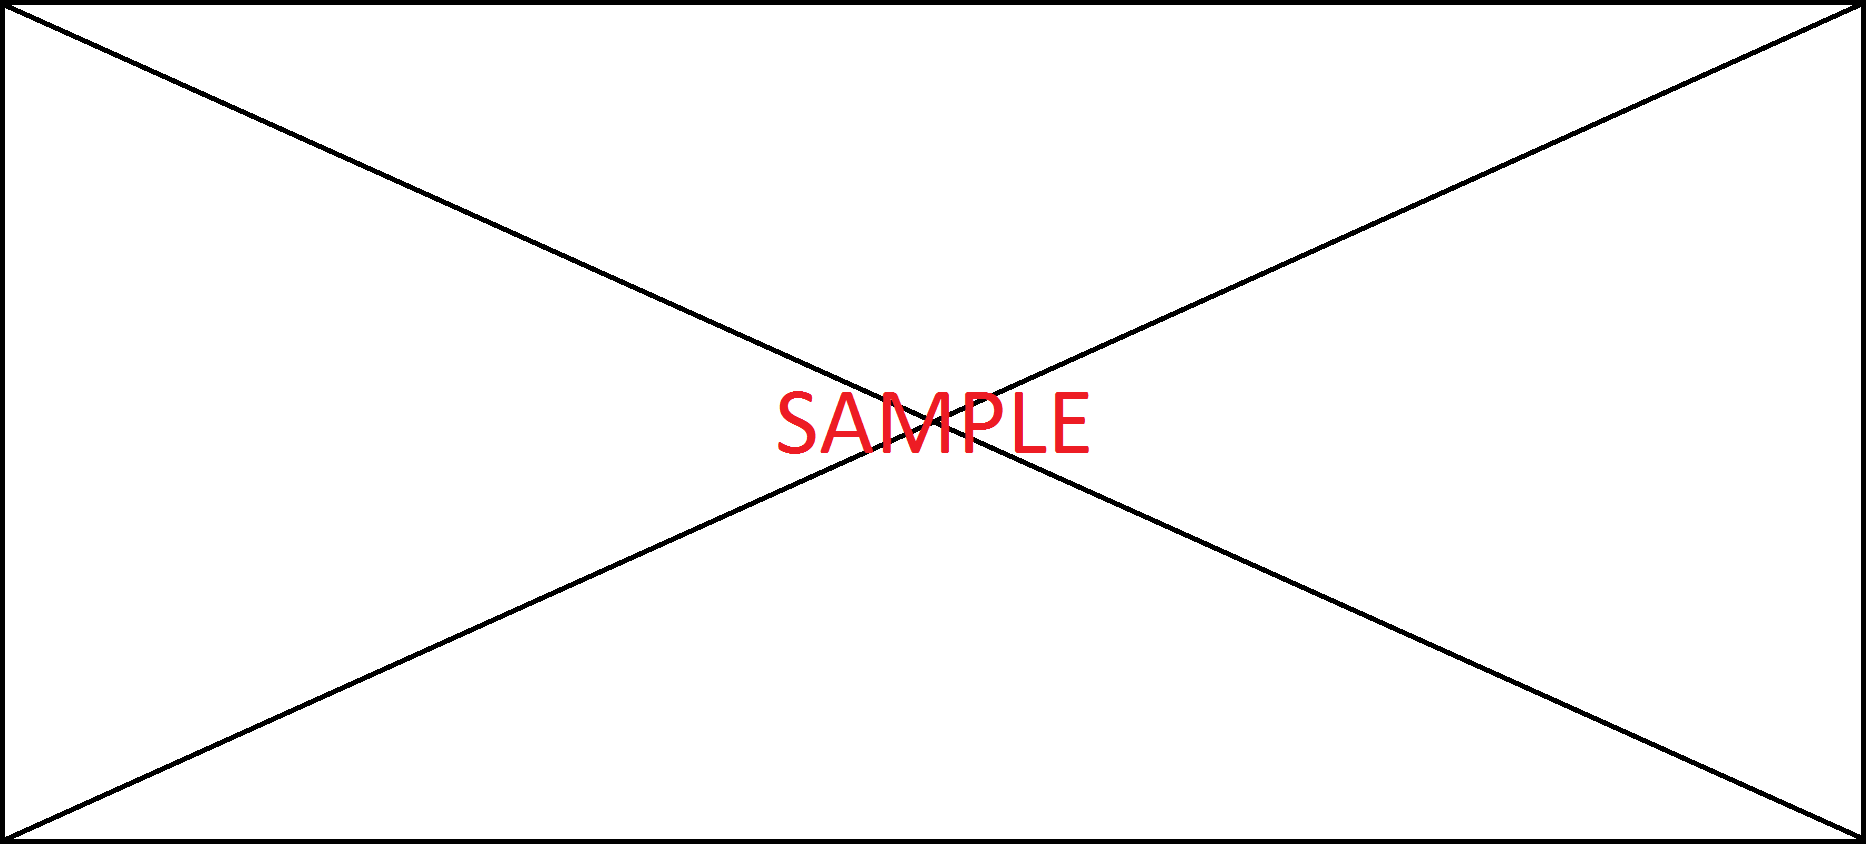
\includegraphics[width=\textwidth, height=\measurepage]{img/fill_page}}

\pagestyle{fancy}
\fancyhead{}
\fancyhead[C]{PML30 Saint-Petersburg}
\fancyfoot{}
\fancyfoot[R]{\thepage}
\fancyfoot[C]{Россия, Санкт-Петербург, Физико-математический Лицей №30. 2014-2015}

\fancypagestyle{titlestyle}
{
   \fancyhead{}
   \fancyfoot{}
   \renewcommand{\footrulewidth}{0.0 mm}
   \renewcommand{\headrulewidth}{0.0 mm}
}

\title{ Техническая книга, ФМЛ №30, команда ${\varphi}$}

\begin{document}
\thispagestyle{titlestyle}
   \begin{titlepage}
      \newpage

      \begin{center}
         \LARGE\textit{Центр робототехники \\ Физико-Математический Лицей №30}

         \vspace{8em}

         \LARGE{Техническая книга \\ Соревнований First FTC}

         \vspace{4em}

         Команда \\ PML30 (${\varphi}$)

      \end{center}
   \end{titlepage}

   \newpage
   \large Состав команды:

   \begin{flushleft}
      \emph{Капитан: Фокин Иван} \\
      \emph{Радионов Максим} \\
      \emph{Сафронов Никита} \\
      \emph{Максимычев Евгений}
   \end{flushleft}

   \large Руководители:

   \begin{flushleft}
      \emph{Федотов Антон Владимирович} \\
      \emph{Крылов Георгий Андреевич} \\
      \emph{Лузин Дмитрий Валерьевич} \\
      \emph{Лузина Екатерина Павловна}
   \end{flushleft}   

   \newpage
   \tableofcontents{}

   \newpage

   \section{Инженерный раздел}
   \subsection{Концепция робота}
   \subsubsection{Конструкция}
   \begin{itemize}
      \item Робот должен быть мобильным, двигаться быстро и, по возможности в любом направлении (имеется в виду способность двигаться боком).
      \item Робот должен быть снабжен датчиками угла оборота (энкодерами) для лучшей управляемости в автономном периоде.
      \item Робот должен быть компактным и не занимать лишнего места, чтобы не мешать союзнику по альянсу, а также для удобства транспортировки.
      \item Робот должен быть способен управлять пятью (5) мячами одновременно.
      \item Робот должен иметь приспособление для перемещения подвижных корзин.
      \item По возможности робот должен быть легким, чтобы его было легче переносить
      \item Конструкция робота должна обеспечивать быстрый доступ ко всем его ключевым узлам.
   \end{itemize}
   \subsubsection{Автономный период}
     \begin{itemize}
        \item Робот должен иметь несколько версий автономного периода, в зависимости от того, где он стартует и каковы возможности союзника по альянсу.
        \item Программа автономного периода должна быть по возможности простой.
        \item По возможности должна быть реализована программа, дающая роботу возможность ориентироваться по ИК-датчику.
     \end{itemize}
     \subsubsection{Управляемый период}
       \begin{itemize}
          \item Управление роботом должно быть простым, удобным и интуитивно понятным.
          \item Один оператор полностью отвечает за перемещение робота, а второй - за все остальное.
          \item Некоторые действия в управляемом режиме могут управляться автономно, для того, чтобы снять лишнюю нагрузку с оператора.
          \item Желательно, чтобы у оператора была возможность управления скоростью робота, поскольку совершать точные манипуляции с игровыми элементами на максимальной скорости довольно трудно.
       \end{itemize}

      \fillpage

     \subsection{Стратегия} 
        \subsubsection{Автономный период}
          \begin{enumerate}
             \item Положить два автономных мяча в две разные корзины (подвижные либо центральную).
             \item Взять как можно больше передвижных корзин и отвезти их в зону парковки.
             \item По пути в зону парковки по возможности задействовать механизм высвобождения мячей.
             \item В зоне парковки поднять корзины над полем.         
          \end{enumerate}
         \subsubsection{Управляемый период-основная часть}
         \begin{enumerate}
            \item Отпустить подвижные корзины и обеспечить к ним свободный доступ союзника по команде. Но приэтом возить за собой одну корзину для того, чтобы не тратить много времени на перемещение мячиков в корзину
            \item Наполнять мячами сначала 90-сантиметровую корзину, затем, если она заполнится, переходить к 60-сантиметровой и 30-сантиметровой.
            \item Избегать столкновений, как с союзником, так и с противниками, поскольку из-за этого теряется время.
         \end{enumerate}
         \subsubsection{Управляемый период - финал}
         \begin{enumerate}
         \item Сознательно отказаться от заполнения мячами центральной корзины, оставив это союзнику по альянсу.
         \item Отвезти как можно больше передвижных корзин на пандус.
         \item Заехать роботом на пандус 
         \end{enumerate}
         \subsection{Планируемые этапы создания робота}
         \begin{enumerate}
            \item Создание колесной (или гусеничной) базы робота.
            \item Создания программы для управления колесной базой с помощью одного (1) джойстика.
            \item Создания системы контроля мячей.
            \item Создание программы для управления системой контроля мячей параллельно с движением робота с помощью двух (2) джойстиков.
            \item Написание программы для автономного периода.
            \item Создание системы поднятия союзника, а также других возможных дополнительных систем, таких как декоративная светодиодная подсветка.
            \item Установка на робота дополнительной защиты корпуса для предотвращения повреждений при случайных столкновениях.
            \item Тренировки как в одиночку, так и с другими роботами (при их наличии).
            9.   Внесение доработок п итогам первых соревнований.
         \end{enumerate}

         \fillpage

         \subsection{Общекомандные собрания}
         \subsubsection{29.09.14}
         \begin{enumerate}
            \item Время начала и окончания собрания:
            \newline
            18:00 - 21:30
            \item Цели собрания:
            \newline
            1. Обсудить правила FTC \newline
            2. Разобрать основные аспекты конструкции робота.\newline
            3. Разработать стратегию игры нашей команды.\newline
            \item Проделанная работа:
            \newline
         3.1.Была обсуждена 2 часть правил, с которыми каждый из нас предварительно ознакомился самостоятельно.\newline
            3.2.    В ходе обсуждения конструкции робота было выдвинуто несколько идей:\newline
            3.2.1.   Размеры робота:\newline
            3.2.1.1.   Робот должен быто достаточно компактным, чтобы помимо самого корпуса в размеры помещался еще и захват для мячей.\newline
            3.2.1.2.   Робот должен быть компактным, чтобы не мешать союзникам.\newline
            3.2.1.3.   Корпус робота не должен быть слишком маленьким, иначе он будет неустойчив в разложенном состоянии с вытянутым ковшом (максимальная высота поднятия – 120 см).\newline
            3.2.2.   Колесная база:\newline
            3.2.2.1.   Конструкция с двумя гусеницами. Плюсы данной конструкции заключаются в том, что она отлично ездит по прямой  и разворачивается на месте вокруг точки пересечения диагоналей прямоугольника, в углах которого располагаются катки. Минусами системы являются большие размеры и ненадежность, поскольку гусеница может слететь в самый ответственный момент. Кроме того, в нашем наборе TETRIX отсутствуют гусеницы, поэтому в случае выбора данной конструкции их предстоит сделать самостоятельно.\newline
            3.2.2.2.   Конструкция с четырьмя ведущими колесами, центры которых находятся в углах квадрата. Такая система также хорошо ездит по прямой и разворачивается на месте, но в отличие от предыдущей занимает значительно меньше места и практически неразрушаема, что имеет важную роль в соревнованиях FTC.\newline
            3.2.2.3.   Конструкция с четырьмя ведущими омни-колесами из набора TETRIX, центры которых находятся в углах квадрата, расположенными под углом в 45 градусов к корпусу. Превосходство данной конструкции над предыдущими в том, что она способна двигаться не только вперед или назад, а во всех направлениях. Эта конструкция позволяет роботу очень быстро поворачиваться на месте, но плохо показывает себя при движении по прямой, что может негативно сказаться на автономном периоде.\newline
            3.2.2.4.    Конструкция с четырьмя ведущими омни-колесами, в которых ролики располагаются под углом в 45 градусов к направлению вращения колеса, центры которых находятся в углах квадрата, таким же образом, как в случае с обычными колесами. Плюсы: точное движение по прямой, быстрый разворот на месте, возможность движения в любом направлении без поворота корпуса. Минусы: относительно сложная программа управления колесами, необходимость докупать колеса отдельно в связи с отсутствием таковых в наборе.
            3.2.3.   Система контроля мячей:
            3.2.3.1.   Корзина для шаров закреплена на вертикальных раздвижных мебельных рейках, основание которых жестко зафиксировано на каркасе робота, а механизм раздвигания приводится в действие DC-мотором, наматывающим на себя леску. Плюсы: простота и надежность конструкции (за исключением лески), высокая точность подъема корзины-захвата на заданную высоту. Минусы: леска способна порваться в ходе соревнований\newline
            3.2.3.2.   Корзина для шаров закреплена на раздвижных мебельных рейках, механизм раздвигания которых приводится в действие DC-мотором, наматывающим на себя леску, а основание установлено на оси другого DC-мотора, способного поворачивать ее в вертикальной плоскости, параллельной длине робота. Плюсы: возможность раздвигания системы в горизонтальном положении снимает часть нагрузки с лески, точность подъема корзины-захвата на заданную высоту средняя. Минусы: леска способна порваться в ходе соревнований.\newline
            3.2.3.3.   Корзина для шаров закреплена на системе из некоторого количества реек, соединенных между собой сервоприводами. Плюсы: отсутствие лески, способной порваться в ходе соревнований. Минусы: чрезмерная сложность и громоздкость конструкции вкупе с ее весьма сомнительной надежностью.\newline
            3.2.4.   Система фиксирования подвижной корзины (для более точного закидывания мячей в корзину, а также для транспортировки ее в зону парковки):\newline
            3.2.4.1.   П-образный захват с двумя сервоприводами, фиксирующими корзину между балками, установленный на оси DC-мотора, способного поворачивать ее в вертикальной плоскости, параллельной длине робота. Плюсы: способность поднимать корзины над полом, входит в размеры в сложенном состоянии. Минусы: занимает много места.\newline
            3.2.4.2.   Такой же захват, только вместо балок-клешней используются крючки, способные захватывать корзину за отверстия, расположенные в ее основании. Плюсы: компактнее предыдущего варианта. Минусы: Попадать крючками в отверстия будет довольно трудно.\newline
           \item Итоги собрания:
           \newline
           4.1.   В результате обсуждения были сформированы общие идеи, касающиеся нашего проекта. Они были помещены в разделы «Концепция робота»,  «Стратегия» и «Планируемые этапы создания робота».\newline
           4.2.   Было определено общее направление приложения усилий, однако ничего конкретного пока решено не было.
           \newline
           \item Задачи для следующего собрания:
           \newline
           5.1.Выбрать оптимальную колесную базу.\newline
           5.2.Выбрать оптимальный размер корпуса робота, исходя из соображений компактности и устойчивости.\newline
           5.3.Выбрать наилучшую систему контроля шаров.\newline
           5.4.Выбрать наиболее эффективный вид фиксирования подвижной корзины.\newline      
         \end{enumerate}
         
         \fillpage
         
         \subsubsection{1.10.14}
         \begin{enumerate}
            \item Время начала и окончания собрания:
            \newline
            18:00 - 21:30
            \item Цели собрания:
            \newline
            2.1.   Выбрать и сделать колесную базу робота.\newline
            2.2.   Создать простейшую программу для управления им с джойстика\newline
            \item Проделанная работа:
            \newline
            3.1.Была создана колесная база робота:\newline
            3.1.1.   Предпочтение было отдано варианту с омни-колесами с роликами, расположенными под углом в 45 градусов к направлению вращения, однако, поскольку пока у нас в наличии их не было, вместо омни-колес было решено установить обычные колеса из набора TETRIX.\newline
            3.1.2.   Для обеспечения устойчивости робота наиболее тяжелые компоненты были расположены как можно ближе к земле. Таким образом, в нижней части робота был расположен аккумулятор (он, как самая тяжелая деталь робота, был помещен в заднюю часть для того, чтобы уравновесить захват мячей, который будет располагаться в передней части робота), микроконтроллер NXT и драйвера моторов и сервоприводов.\newline
            3.1.3.   Поскольку вся управляющая электроника была размещена у самого пола, провода могли случайно вылезти наружу с нижней части и зацепиться за других роботов или за собственные подвижные части, поэтому на следующее занятие было решено принести пластмассовую папку и вырезать из нее кусок для днища нужного размера, чтобы защитить управляющую электронику с проводами с нижней части.\newline
            3.2   Была выдвинута идея сделать подъемник для мячей по принципу конвейера. Такая система позволила бы установить захват мячей стационарно на корпусе робота, а поднимать только сами мячи. Вот идеи конвейеров:\newline
            3.2.1.   Лента с корзинами, расположенными на ней через равные промежутки.\newline
            3.2.2   Раздвижной полый цилиндр, внутри которого перемещаются оси, выполняющие роли основания корзины, стенками которой являются стенки раздвижного цилиндра.\newline
            3.2.3.   Раздвижной полый цилиндр, внутри которого с одной стороны расположена движущаяся вверх лента с закрепленными на ней упругими «ворсинками», проталкивающими шары вверх по трубе. Плюс данной системы в том, что мячи могут захватываться лентой сразу, а не ждать следующую корзину.
            \newline
            \item Итоги собрания:
            \newline
            4.1.   Колесная база робота собрана.\newline
            4.2.   Программа управления роботом не реализована
            \newline
            \item Задачи для следующего собрания:
            \newline
            5.1. Создать программу управления роботом.\newline
            5.2. Установить защиту днища
            \newline   
         \end{enumerate}

         \fillpage

         \subsubsection{6.10.14}
         \begin{enumerate}
            \item Время начала и окончания собрания:
            \newline
            21:00 - 21:30
            \item Цели собрания:
            \newline
            Начать писать программу для управления роботом с джойстика
            \item Проделанная работа:
            \newline
            3.1.   Для проверки способностей ходовой было написано две программы движения робота – по прямой и вокруг своей оси. При движении по прямой робот показал блестящие результаты, поскольку почти не отклонился от изначальной траектории за все время движения. При вращении вокруг своей оси робот сильно дребезжал, поскольку из-за высокого коэффициента трения его колеса не могли проскальзывать по полу и подпрыгивали, но в целом это никак не влияло на точность поворота. Робот вращался точно вокруг своего центра тяжести, однако последний находился не в центре робота, а ближе к задней части. Возможно, для удобства управления следует переместить центр тяжести ближе к линии пересечения диагоналей квадрата, в углах которого расположены колеса. Тогда место, необходимое на разворот, будет меньше и мы будем меньше мешать союзникам.\newline
            3.2.   В результате обсуждения типа подъемника был выбран вариант с раздвижными мебельными рейками, основание которых жестко зафиксировано на каркасе робота. Эта конструкция наиболее надежная из всех описанных выше, а также самая простая в исполнении.
            \newline
            \item Итоги собрания:
            \newline
            4.1.   Программа управления с джойстика пока не реализована.\newline
            4.2.   Выбран тип подъемника для мячей.
            \newline
            \item Задачи для следующего собрания:
            \newline
            Купить мебельные рейки для создания подъемника
         \end{enumerate}

         \fillpage

         \subsubsection{07.10.2014}
         \begin{enumerate}
            \item Время начала и окончания собрания:
            \newline
            17:00 – 21:30
            \item Цели собрания:
            \newline
            2.1.    Написать программу для управления роботом с джойстика.\newline
            2.2.   Начать создание подъемника для шаров.
            \item Проделанная работа:
            \newline
            3.1.   Сегодня было реализовано управление роботом с помощью джойстика. Управление моторами осуществлялось с помощью левого аналогового датчика. В ходе испытаний было выяснено, что когда на моторы подается малый ток, они не могут провернуться, и издают громкий неприятный звук, вероятно свидетельствующий о том, что они работают на износ. В связи с этим было решено поставить ограничение на подачу моторам слишком слабого сигнала.\newline
            3.2.   Для того, чтобы поднимать корзину на 120 см, было решено собрать две направляющих, каждая из которых состоит из четырех мебельных реек, двух по 30 см и двух по 35 см. Таким образом, рабочая высота составила 130 см. Направляющие были установлены на робота, однако каким образом будет реализован механизм для их раздвигания пока неизвестно.\newline
            3.3.   Поскольку во внутренней части робота оставалось много свободного пространства, было решено установить подъемник шаров в центральной части робота, а управляющую электронику переместить в заднюю часть робота и закрепить ее там для предотвращения ее повреждения расположенным рядом механизмом подъема шаров. В передней части робота было оставлено место для корзины. \newline
            3.4.   Поскольку корзина будет опускаться внутри робота, она будет защищена от столкновений с другими роботами. Но в таком случае встает вопрос о том, как мячи будут попадать в корзину, если она будет располагаться внутри робота. Для решения данной проблемы было решено увеличить расстояние между полом и нижней частью передней балки каркаса до 7 см, чтобы в него мог пройти большой шарик. Этого удалось добиться поворотом моторов вокруг своей оси в местах их крепления из положения, в котором вал находится сверху в положение, в котором вал находится сбоку. Кроме того, такое решение позволило отдалить колеса друг от друга, несколько увеличив устойчивость робота.\newline
            3.5.   Впоследствии в передней части робота было решено установить мягкие щетки, подобные тем, которые устанавливаются на снегоуборочные машины, которые будут вращаться и захватывать мячи. В случае, когда робот собрал максимальное количество шариков, оператор сможет остановить вращение щеток, что не даст другим мячам случайно попасть в ковш.
            \item Итоги собрания:
            \newline
            4.1.   Реализована простейшая программа по управлению роботом, нуждающаяся в доработке.\newline
            4.2.   Созданы и закреплены на роботе направляющие для подъемника.\newline
            4.3.   Батарея и драйверы моторов надежно зафиксированы на роботе, блок NXT не был закреплен, поскольку его периодически требуется вынимать для замены аккумулятора.\newline
            4.4.   Увеличен клиренс робота.\newline
            
            \item Задачи для следующего собрания:
            \newline
            5.1.   Доработать программу управления роботом.
            5.2.   Реализовать управление роботом по Bluetooth.\newline
            5.3.   Разработать механизм раздвигания направляющих.
         \end{enumerate}
         \newpage
         \subsubsection{08.10.2014}
         \begin{enumerate}
            \item Время начала и окончания собрания:
            \newline
            18:30 – 21:40
            \item Цели собрания:
            \newline
            2.1.   Написать программу для управления роботом по Bluetooth.\newline
            2.2.   Придумать оптимальный способ приведения подъемника в действие.\newline
            \item Проделанная работа:
            \newline
            3.1.   Программа управления робота была изменена. Было установлено ограничение таким образом, что при слабых отклонениях джойстика робот не реагировал, что позволило во-первых избежать чрезмерной нагрузки на моторы при подаче на них значений, близких к нулю, а во-вторых не допускать неконтролируемого движения робота в результате случайного задевания рукой аналогового датчика.\newline
            3.2.   Было осуществлено подключение к роботу по Bluetooth. \newline
            3.3.   В ходе испытаний была испытана способность робота подниматься по наклонной плоскости. Робот  способен подняться по горке с углом наклона в 30 градусов.\newline
            3.4.   Для подъема раздвижных реек было решено создать конструкцию из восьми поперечных балок, закрепленных попарно между двумя направляющими таким образом, чтобы каждой балке, закрепленной в верхней части неподвижной составляющей одной мебельной направляющей, соответствовала балка, закрепленная в нижней части ее подвижной составляющей. В этом случае трос, закрепленный на нижней балке и перекинутый через верхнюю, при натягивании раздвигает мебельную рейку.\newline
            3.5.   Вместо лески для раздвигания подъемника было решено использовать ремень, поскольку он гораздо надежнее и не запутается в ходе матча.
            \newline
            \item Итоги собрания:
            \newline
            4.1.   Реализовано управление роботом по Bluetooth. Результаты удовлетворительные.\newline
            4.2.   Разработана концепция механизма раздвигания подъемника
            \newline
            \item Задачи для следующего собрания:
            \newline
            5.1.   Приобрести ремень для раздвигания подъемника нужной длины. Длина не менее 3-х метров.\newline
            5.2.   Приобрести алюминиевый профиль для создания креплений для поперечных балок.            
         \end{enumerate}
         \newpage
         \subsubsection{10.10.2014}
         \begin{enumerate}
            \item Время начала и окончания собрания:
            \newline
            16:30 – 21:40
            \item Цели собрания:
            \newline
            2.1.   Выбрать оптимальный диаметр поперечных балок для подъемника.\newline
            2.2.   Распилить алюминиевый профиль на сегменты нужной длины, просверлить в них нужные отверстия и установить их между направляющими вместо прослойки из оригинальной тетриксовской детали
            \newline
            \item Проделанная работа:
            \newline
            3.1.   Был приобретен ремень для раздвигания подъемника.\newline
            3.2.   Для создания креплений для поперечных балок была приобретена алюминиевая полоса размерами 200 см х 5 см х 0,2 см.\newline
            3.3.   В качестве поперечных балок в наборе TETRIX были доступны цилиндрические валы диаметром 15 мм и оси для колес диаметром 5 мм. Предпочтение было отдано последним по причине их большей компактности.\newline 
            3.4.   Поскольку оси меньшего диаметра имели срезанный край для закрепления втулок колес, они оказывали большое сопротивление движению ремня из-за трения. Тогда было решено насадить на ось свободные (без креплений) втулки. Предварительные испытания продемонстрировали полную состоятельность данной идеи.\newline
            3.5.   После этого было решено приступить к действиям:\newline
            3.5.1.   Направляющие подъемника были предварительно разобраны.\newline
            3.5.2.   Алюминиевая полоса была распилена на 6 сегментов: 2 по 30 см и 4 по 35 см.\newline
            3.5.3.   При сверлении полученных деталей возникли трудности, поскольку все сверла оказались сточенными. К следующему занятию было решено купить новые сверла
            \newline
            \item Итоги собрания:
            \newline
            4.1.   Выбраны балки для подъемника.\newline
            4.2.   Балка распилена на сегменты нужной длины.\newline
            4.3.   Просверлить отверстия не удалось.
            \newline
            \item Задачи для следующего собрания:
            \newline
            5.1.   Купить новые сверла по металлу.
         \end{enumerate}
         \newpage
         \subsubsection{11.10.2014}
         \begin{enumerate}
            \item Время начала и окончания собрания:
            \newline
            16:40 – 21:40
            \item Цели собрания:
            \newline
            2.1.   Просверлить отверстия в креплениях для балок в подъемнике.\newline
            2.2.   Полностью собрать направляющие подъемника с новыми креплениями.\newline
            2.3.   По возможности установить направляющие на робота
            \newline
            \item Проделанная работа:
            \newline
            3.1. Все крепления были закончены и установлены на направляющие.\newline
            3.2.   При установке креплений для балок на направляющие выяснилось, что алюминиевый профиль тоньше, чем деталь из TETRIX-а, и из-за этого винты, которыми скреплялись направляющие, дальше выходили из отверстий и мешали мебельным рейкам раздвигаться. Было принято решение несколько сточить винты. Поскольку стачивание винта со стороны резьбы могло помешать нормальному ходу гайки по резьбе, была сточена часть шляпки, под которую затем было подложено две гайки. После этого раздвиганию направляющих ничего не мешало.
            \item Итоги собрания:
            \newline
            4.1.   Направляющие собраны, но не установлены на робота.
            \item Задачи для следующего собрания:
            \newline
            5.1.Установить направляющие на робота, собрать полноценный подъемник и испытать его в действии.
         \end{enumerate}
         \newpage
         \subsubsection{13.10.2014}
         \begin{enumerate}
            \item Время начала и окончания собрания:
            \newline
            21:00 – 21:30
            \item Цели собрания:
            \newline
            2.1.   Установить направляющие на робота.\newline
            2.2.   Разработать концепцию механизма для закидывания мячей в подвижные корзины.
            \item Проделанная работа:
            \newline
            3.1.   Поскольку в нашу стратегию входило возить подвижную корзину за собой сзади, было решено установить на последней направляющей ось, вокруг которой мог бы вращаться ковш с мячами. Сверху ковша будет помещена трубка диаметром чуть больше диаметра большего шарика, которая будет поворачиваться вокруг оси вместе с ним и в тот момент, когда ковш будет находиться выше трубки, мячи по ней будут скатываться назад, за робота, туда, где расположена корзина.\newline
            3.2.   Было подсчитано, что оптимальным местом расположения оси, вокруг которой должен будет вращаться ковш, является помещение ее в 20 сантиметрах от нижнего края последнего сегмента направляющих. Дополнительный прирост высоты подъема ковша позволил отказаться от одной пары 30-сантиметровых мебельных реек. Таким образом, у нас осталось три пары мебельных реек рабочей высотой в 105 сантиметров и механизм для закидывания мячей в корзины, находящийся на стадии разработки.\newline
            3.3.   Измененные направляющие были установлены на робота.\newline
            3.4.   После установки направляющих было решено протестировать работу подъемника. Ремень хорошо справлялся с задачей, однако оси прогибались, испытывая сильные нагрузки, из чего был сделан вывод, что нам необходимы более прочные оси. Кроме того, рейки раздвигались неодинаково, поэтому было решено попарно жестко скрепить  их друг с другом. Критических проблем в системе подъемника обнаружено не было.
            
            \item Итоги собрания:
            \newline
            4.1.   Направляющие установлены на робота. Их конструкция упрощена.\newline
            4.2.   Разработана концепция механизма закидывания мячей в корзины.
            
            \item Задачи для следующего собрания:
            \newline
            5.1.   Собрать устройство для вращения ковша.
            5.2.   Найти и купить более прочные оси для подъемника.\newline
            5.3.   Купить еще один алюминиевый профиль для жесткого закрепления мебельных направляющих между собой.
            
         \end{enumerate}
         \newpage
         \subsubsection{15.10.2014}
         \begin{enumerate}
            \item Время начала и окончания собрания:
            \newline
            15.10.2014
            \item Цели собрания:
            \newline
            2.1.   Заменить перекладины на подъемнике на более прочные.\newline
            2.2.   Скрепить попарно направляющие в подъемнике для того, чтобы он ровно раздвигался.
            
            \item Проделанная работа:
            \newline
            3.1.   У нас не было возможности приобрести необходимые ресурсы для доработки подъемника, поэтому сегодня было решено заняться разработкой захвата для мячей в виде вращающейся щетки.\newline
            3.2.   Передняя часть робота была видоизменена и на ней были поставлены сервопривод свободного вращения с осью, на которой было решено закрепить щетку, в качестве ворсинок которой будут использоваться стяжки.
            
            \item Итоги собрания:
            \newline
            4.1.   Создана основа захвата для мячей.\newline
            4.2.   Доработка подъемника не осуществлена
            
            \item Задачи для следующего собрания:
            \newline
            5.1.   Купить все необходимые ресурсы для доработки подъемника.\newline
            5.2.   Доделать захват для мячей и написать программу для управления им.
            
         \end{enumerate}
         \newpage
         \subsubsection{16.10.2014}
         \begin{enumerate}
            \item Время начала и окончания собрания:
            \newline
            17:10 – 21:00
            \item Цели собрания:
            \newline
            2.1.   Подключить контроллер для сервоприводов и подсоединить к нему сервопривод захвата.\newline
            2.2.   Включить в программу управления роботом управление захватом.\newline
            2.3.   Доработать подъемник.
            
            \item Проделанная работа:
            \newline
            3.1.   К сегодняшнему занятию мы приобрели алюминиевую полосу 100 см х 4 см х 0,3 см для создания поперечных перекладин для попарного скрепления направляющих и алюминиевую ось длиной 100 см и диаметром 8 мм для создания перекладин, за которые будет цепляться подъемник.\newline
            3.2.   Полоса была распилена на 4 сегмента нужной длины. Для того чтобы установить получившиеся поперечные ребра жесткости на робота, было решено приобрести Г-образный профиль и распилить его на уголки нужного размера.\newline
            3.3.   Метровой оси хватило на 4 перекладины из необходимых 6. Две из них были закреплены с помощью деталей из набора TETRIX. Для еще одной были просверлены отверстия, однако она не была жестко закреплена. Последнюю ось, предназначенную для самой внутренней пары направляющих, было решено пока не устанавливать: во-первых, мы пока не придумали, как это сделать, а во-вторых это бы осложнило доработку подъемника.\newline
            3.4.   Нами был установлен контроллер сервоприводов и к нему был подключен сервопривод свободного вращения, отвечающий за захват мячей.\newline

            \item Итоги собрания:
            \newline
            4.1.   Установлен контроллер сервоприводов.
            \newline
            4.2.   Программа управления сервоприводом не написана.\newline
            4.3.   Алюминиевая полоса распилена на ребра жесткости, готовые к закреплению на роботе.\newline
            4.4.   Ось распилена на перекладины.
            
            \item Задачи для следующего собрания:
            \newline
            5.1.   Купить еще одну алюминиевую ось и напилить из нее оставшиеся перекладины.
            \newline
            5.2.   Купить Г-образный профиль и сделать из него уголки для закрепления ребер жесткости на подъемнике.
         \end{enumerate}
         \newpage
         \subsubsection{17.10.2014}
         \begin{enumerate}
            \item Время начала и окончания собрания:
            \newline
            17:00 – 20:00
            \item Цели собрания:
            \newline
            2.1.   Написать программу управления захватом и включить ее в программу управления роботом.
            \item Проделанная работа:
            \newline
            3.1.   Была написана программа управления сервоприводом. По нажатию кнопки привод включается, а после того, как оператор убирает руку с кнопки, он останавливается. Во время испытаний стало понятно, что такая система неудобна для оператора, поскольку ему нужно постоянно держать руку на кнопке. На данный момент все команды подаются с одного джойстика, но впоследствии у первого оператора останутся только обязанности управления движением, а все остальное будет делать оператор №2.\newline
            3.2.   При испытании тестовой версии захвата на банках (мячей у нас на тот момент не оказалось) выяснилось, что он вместо того, чтобы захватывать их, он их отталкивает. Мы поняли, что стяжки закреплены на оси сервопривода не той стороной и решили их переставить, но пока не стали этого делать.  \newline
            3.3.   Кроме того, было решено перенести переднюю поперечную балку дальше от оси для того, чтобы она не препятствовала движению щеток-стяжек.\newline
            3.4.   Закреплять стяжки на оси было решено с помощью термоклея, но так как на этом занятии его у нас не было, мы решили отложить все до завтра
            \newline
            \item Итоги собрания:
            \newline
            4.1.   Написана простейшая программа для управления захватом.\newline
            4.2.   Захват испытан в действии. Разработаны идеи его усовершенствования.
            
            \item Задачи для следующего собрания:
            \newline
            5.1.   Создать окончательную версию захвата.\newline
            5.2.   Изменить программу управления захватом на более удобную
            
         \end{enumerate}
         \newpage
         \subsubsection{18.10.2014}
         \begin{enumerate}
            \item Время начала и окончания собрания:
            \newline
            16:30 – 21:40
            \item Цели собрания:
            \newline
            2.1.   Создать окончательную версию захвата.\newline
            2.2.   Изменить программу управления захватом на более удобную
            
            \item Проделанная работа:
            \newline
            3.1.   Поперечная балка передвинута дальше от оси вращения захвата.\newline
            3.2.   Стяжки размещены на оси в 4 ряда через каждые 90° и закреплены термоклеем.\newline
            3.3.   Программа управления захватом заменена. Теперь сервопривод меняет свое состояние (стоит или работает) по нажатию кнопки. Это позволяет оператору не отвлекаться на поддержание захвата в работающем состоянии.\newline
            3.4.   Были проведены полноценные испытания захвата с двумя мячами из набора NXT диаметром 5 см. Испытания прошли успешно, робот был способен захватывать мячи, расположенные как на открытом пространстве, так и возле стены. Некоторое неудобство доставлял тот факт, что щетка захвата расположена не вдоль всей передней кромки робота, а только посередине, поэтому для захвата мяча требовалось к нему прицеливаться. Впоследствии мы планируем устранить этот недостаток, установив по бокам от захвата балки, расположенные в виде воронки, что позволит шарикам самостоятельно закатываться в область действия захвата.\newline
            3.5.   При программировании сервопривода свободного вращения выяснилось, что при постановке его на нейтраль он стремится удерживать угол, из-за чего начинает дребезжать. Этот баг необходимо исправить.\newline
            3.6.   Было замечено, что ограничители хода мебельных реек не выдерживают массы подъемника и подвижные части реек проваливаются. В связи с этим требуется укрепить данные ограничители без ущерба подвижности  реек.
            
            \item Итоги собрания:
            \newline
            4.1.   Завершена работа над механизмом захвата.\newline
            4.2.   Создана удобная программа для управления захватом
            
            \item Задачи для следующего собрания:
            \newline
            5.1.   Исправить баг с сервоприводом свободного вращения.   \newline
            5.2.   Укрепить ограничители хода мебельных реек.   \newline
            5.3.   Установить балки помощи захвату
            
         \end{enumerate}
         \newpage
         \subsubsection{20.10.14}
         \begin{enumerate}
            \item Время начала и окончания собрания:
            \newline
            20:30-21:30
            \item Цели собрания:
            \newline
            2.1. Устранить баг сервопривода
            \newline
            2.2.Закрепить ребра жесткости на подъемнике
            \item Проделанная работа:
            \newline
            3.1. Для устранения бага с сервоприводом мы попробовали сделать так, чтобы перед остановкой он немного прокручивался назад.Однако это ни к чему не привело\newline
            3.2. Приобретенный Г-образный профиль распилен на уголки нужной длины\newline    
            3.3.  Ребра жесткости для подъемника изготовлены и частично закреплены

            \item Итоги собрания:
            \newline
            4.1. Баг сервопривода не устранен
            \newline
            4.2. Все готово для закрепления ребер жесткости на направляющие подъемника\newline
            4.3. Одно ребро жесткости установлено
            \item Задачи для следующего собрания:
            \newline
            5.1. Закончить закрепление ребер жесткости на подъемник\newline
            5.2. Устранить баг сервопривода
         \end{enumerate}
         \newpage
          \subsubsection{21.10.14}
          \begin{enumerate}
             \item Время начала и окончания собрания:
             \newline
             17:00-19:00
             \item Цели собрания:
             \newline
             2.1. Еще раз обдумать стратегию автономного и финального периодов и в случае необходимости внести поправки\newline
             2.2. Закончить установку ребер жесткости на направляющие подъемник\newline
             2.3. Установить нижние ограничители для мебельных реек\newline
             \item Проделанная работа:
             \newline
             3.1. Ребра жесткости установлены на подъемник\newline
             3.2. Устранена проблема проваливания реек путем укрепления стандартных ограничителей термоклеем\newline
             3.3. Была еще раз обдумана стртегия автономного и финального периодов. Поправок внесено не было\newline
             3.4. В конце собрания произошла поломка одной из мебельных реек (выскочила верхняя часть). Это необходимо исправить
             \item Итоги собрания:
             \newline
             4.1. Все ребра жесткости установлены\newline
             4.2. Установлены нижние ограничители мебельных реек
             \item Задачи для следующего собрания:
             \newline
             5.1.Исправить поломку рейки, понять в чем ее причина и как этого избежать в дальнейшем
          \end{enumerate} 
          \newpage
           \subsubsection{22.10.14}
           \begin{enumerate}
              \item Время начала и окончания собрания:                          
              \newline
              18:00 – 21:40
              \item Цели собрания:
              \newline
              2.1.   Разобраться, в чем причина поломки направляющей.\newline
              2.2.   Отремонтировать направляющую.\newline
              2.3.   Понять, каким образом можно не допустить подобной поломки в дальнейшем
              
              \item Проделанная работа:
              \newline
              3.1.   После тщательного исследования конструкции подъемника было выяснено, что поломка произошла вследствие создания избыточного напряжения из-за стягивания двух направляющих друг с другом поперечным ребром жесткости. Было решено увеличить расстояние между двумя соответствующими направляющими, заменив прослойку между ребром жесткости и направляющими с шайб на более толстые гайки.\newline
              3.2.   Починить мебельную рейку не удалось, поэтому она была заменена на точно такую же, оставшуюся после отказа от лишней пары реек при создании подъемника.\newline
              3.3.   После того, как ребро жесткости было закреплено на роботе так, что прослойки из гаек были поставлены с обоих сторон, было обнаружено, что теперь направляющие слишком сильно распираются поперечной балкой. Тогда было решено оставить гайки только с одной стороны, в то время как с другой вернуть изначальную прослойку из шайб. После этого было достигнуто состояние, в котором направляющие не испытывают негативного поперечного воздействия.\newline
              3.4.   Не смотря на то, что проблема была устранена, на всякий случай было решено приобрести запасные направляющие, поскольку сломанные рейки уже не поддаются восстановлению.\newline
              3.5.   Помимо всего прочего, было создано крепление для перекладины, которая будет располагаться на внутренней паре реек.
              
              \item Итоги собрания:
              \newline
              4.1.   Ремонт подъемника выполнен.\newline
              4.2.   Создано крепление для внутренней рейки   
              \item Задачи для следующего собрания:
              \newline
              5.1.   Приобрести запасные мебельные рейки.
           \end{enumerate}
           \newpage
       \subsubsection{24.10.14}
      \begin{enumerate}
       \item Время начала и окончания собрания:
     \newline
     16:00 - 20:00
     \item Цели собрания:
     \newline
     2.1. Устарнить баг сервопривода
     \newline
     2.2. Изготовить из приобретенного нами листа аллюминия и установить откосы для мячей в виде балок, расположенных в форме воронки в передней части робота
     \item Проделанная работа:
     \newline
     3.1. Баг сервопривода устарнен. Причина его возникновения- вращение сервопривода после остановки с небольшой скоростью, которой не хватало на преодоление силы упругости стяжек. Связано это с нерпавильным значением мощности сервопривода в коде (значение, в котором сервопривод не вращается - 127 вместо стоявшем у нас 135)\newline
     3.2. Лист аллюминия распилен на полосы нужной длины и ширины.\newline
     3.3. Откосы установлены на робота и протестированы. Результат положительный.\newline
     3.4 При тестировании откосов было замечено, что при столкновении с жестким препятствием они изгибаются. Для предотвращения этого были установлены упоры выпиленные из аллюминиевой полосы
     3.5. Подготовлены отверстия для установки оставшейся пары поперечных перекладин на подъемнике
     \item Итоги собрания:
     \newline
     4.1.Баг сервопривода устранен\newline
     4.2.Откосы для мячей установлены на робота
     \item Задачи для следующего собрания:
     \newline
     5.1. Спроектировать и создать механизм захвата передвижных корзин
 \end{enumerate}
           \subsubsection{25.10.14}
           \begin{enumerate}
              \item Время начала и окончания собрания:
              16:00 - 20:00
              \newline
              \item Цели собрания:
              \newline
              2.1. Спроектировать и собрать механизм захвата передвижной корзины
              \item Проделанная работа:
              \newline
              3.1.Было рассмотрено 2 варианта исполнения механизма: 1-ый - сервопривод, к которому прикреплен один коней балки, и при вращении сервопривода балка поворачивается и опускается; 2-ой - к заднему краю корпуса робота прикреплена мебельная рейка, соединенная с сервоприводом через леску и опускающаяся при его вращении\newline
              3.2. Предпочтение было отдано второму в силу его большей компактности\newline
              3.3.Мебельная рейка была распилена для уменьшения ее длины\newline
              3.4. На рейке размечены места для сверления отверстий под крепеж. Сам отверстия просверлены не были ввиду отсутствия на тот момент дрели 
              \item Итоги собрания:
              \newline
              4.1. Механизм захвата корзин спроектирован, но не установлен
              \item Задачи для следующего собрания:
              \newline
              5.1. Закончить создание механизма захвата корзин
           \end{enumerate}
           \newpage
            \subsubsection{27.10.14}
            \begin{enumerate}
               \item Время начала и окончания собрания:
               18:00-19:00
               \newline
               \item Цели собрания:
               \newline
               2.1. Закончить работу над механизмом захвата передвижных корзин\newline
               2.2. Совместно обсудить техническую книгу, внести поправки
               \item Проделанная работа:
               \newline
               3.1.От механизма захвата корзин с мебельной рейкой было решено отказаться из-за сложной реализациии необходимости занижения клиренса (для опускания рейки с помощью лески необходимо поставить ось, через которую будет идти леска, в нижней части робота)\newline
               3.2.Была обсуждена техническая книга и внесены необходимые поправки 
               \item Итоги собрания:
               \newline
               4.1.Механизм захвата корзин решено изменить\newline
               4.2.Внесены необходимые поправки в техническую книгу
               \item Задачи для следующего собрания:
               \newline
               5.1. Закончить работу над механизмом захвата корзины
            \end{enumerate}
            \newpage
             \subsubsection{28.10.14}
             \begin{enumerate}
                \item Время начала и окончания собрания:
                17:00 - 19:00
                \newline
                \item Цели собрания:
                \newline
                2.1. Закончить работу над механизмом захвата корзин
                \item Проделанная работа:
                \newline
                3.1. Сервопривод, который вращает балку должен быть закреплен как можно ниже для максимальной точности захвата\newline
                3.2.Решено было закрепить сервопривод следующим образом:просверлить в балке в задней части робота отверстие диаметром с вал сервопривода для того, чтобы разместить сервопривод так, чтобы он не выходил за пределы корпуса робота (иначе робот не укладывался бы в регламентированные размеры) и в то же время мог свободно вращаться\newline
                3.3. Отверстие просверлено
                \item Итоги собрания:
                \newline
                4.1. Придуман и частично реализована схема закрепления сервопривода для механизма захвата корзин
                \item Задачи для следующего собрания:
                \newline
                5.1. Закончить работу над механизмом захвата корзин
             \end{enumerate}
             \newpage
      \section{Перспективы развития и благодарности}

      
      \end{document}